\documentclass{article}

\usepackage{graphicx}
\usepackage{geometry}
\usepackage{array}
\geometry{left=1cm,right=1cm,top=2.5cm,bottom=2.5cm}
\begin{document}
	
\title{Midterm Report}
\author{Wenjia Zhai(wz363), Jiahui Lu(jl3947), Yishan Xiong(yx468)}
\date{}

\maketitle

\begin{abstract}
The stock trading is exciting for its uncertainty, however, for the future practitioner in financial industry, we believe that there are certain rules lying in the numbers. Traditionally, people use linear multifactorial model to predict future stock price to reduce the possible risks and maximize the profit. 

In this project, we are going to use several machine learning models to predict the direction of the stock price, in other words, it is a classification problem with 2 categories: up and down. We plan to utilize efficient models such as neutral network, random tree, decision tree and SVM to achieve our goal.

\end{abstract}

\section{Exploring raw data}
\subsection{Overview}
The stock price we wish to predict is S\&P 500 component stocks. The S\&P 500 stock market index, maintained by S\&P Dow Jones Indices, comprises 505 common stocks issued by 500 large-cap companies and traded on American stock exchanges. \\
Our raw data is come from Wharton database, with a time span of 10 years and 505 stocks. The data contains Daily stock prices, Return values, Trading volumes and The CBOE Volatility Index,.

\subsection{Data Description}
Since we are trying to predict the future stock price, we have graphed the chart pattern of stock price and here are several typical chart patterns: \\
a. Continuous upward trend \\
b. Fluctuating trend \\
c. Continuous downward trend \\
\begin{center}
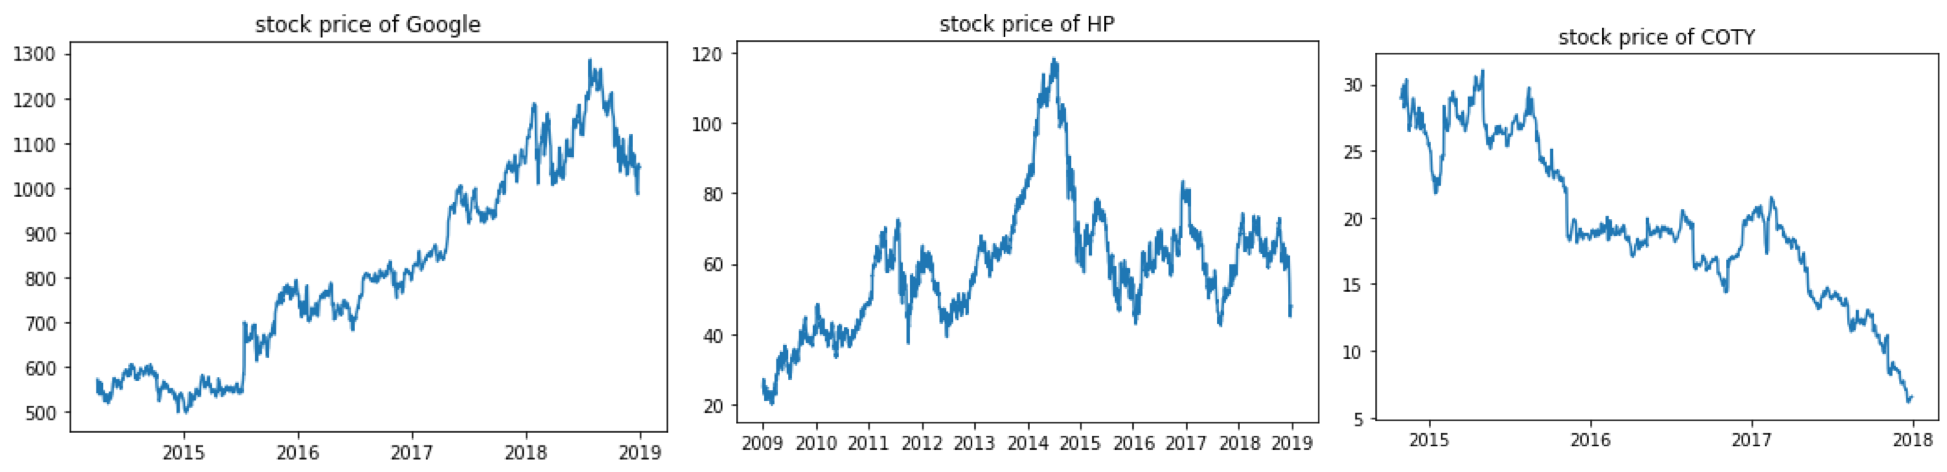
\includegraphics[width=150mm, scale=1]{mid_1.2_4.png}
\end{center}
\subsection{Data cleaning}
When processing the data, we found that our data has unaligned data time and there are some missing data because of suspension of the stock. To deal with the data, we first reset all the data time index with uniform date format. Then we drop nan data because when stock is suspended, there is no need to predict its price will go up or down. For stocks which have more than 10\% missing data points, we drop the entire stock.

\section{Features, preliminary regression and analysis}
To make it easier to find the characteristics of our data, we select one single company with least nans and blanks in our time period. We chose google (NASDAQ:GOOGL) as the stock for data description in the following paragraphs. 
\subsection{Features} 
\subsubsection{Single variable distribution}  
\begin{center}
\begin{tabular}{m{1cm}<{\centering}|m{8cm}<{\centering}|m{8cm}<{\centering}}
Feature & Formula (all features are delayed by 1day in our real calculation) & Description \\
\hline
1 & $\frac{Mean(\frac{(Close-Low)-(High-Close)}{High-Low}*Volume, 20)}{Volume}$ & A measure of the mean intraday level of close price, modified by volume. \\
\hline
2 & $\frac{High-Mean(High,5)}{Mean(High,5)}$ & A comparison between today's high price and the previous mean.  \\
\hline
3 & $\frac{Std(Volume,20)}{Volume}$ & A measure of the monthly volume dispersion.  \\
\hline
4 & $\frac{Ask-Bid}{Delay(Ask,1)-Delay(Bid, 1)}$ & The change of bid-ask spread.\\
\hline
5 & $Corr(Rank(Close), Rank(Volume), 10)$ & The deviation or converge of close price and volume market level. \\
\hline
6 & $\frac{\sqrt{High * LOW} - Close}{Close}$ & A comparison between close price and the “geometric mean” intraday price.  \\
\hline
7 & $1-\frac{Close}{Delay(Close, 5)}$ & A feature to measure the inverse effect of stock price. \\
\hline
8 & $Rank(Std(High, 10))$  & A market level measurement of the fluctuation of high price.\\
\hline
9 & ts\_Max(Corr(ts\_Rank(Volume, 5), ts\_Rank(Close, 5), 5),3) & The time series max of the deviation or converge of close price and volume.\\
\hline
10 & $1-\frac{VWRET}{Delay(VWRET, 5)}$& The value-weighted return change. \\
\hline
11 & $\frac{Std(Close, 5)}{Close}$ & A measure of the weekly close price dispersion. \\
\hline
12 & Corr(High, Volume, 10) & The deviation or converge of high price and volume trend. \\
\hline
13 & $\frac{Std(VWRET, 20)}{VWRET}$ & A measure of the monthly return dispersion. \\
\hline
14 & $Mean(\frac{High}{Low}, 20)$ & A measure of individual stock price volatility.\\
\hline
15 & VIX Index & The CBOE Volatility Index. A popular measure of the stock market's expectation of volatility
\end{tabular}
\end{center}
Here are the distribution of every features(Fig.Feature distribution).  \\
From the picture above, we can see feature 1,2,4,5,6,7,10,11,12,13 look like the normal distribution very much, and feature 3,9,14,15 follow positive skewness distribution. 

\subsubsection{Feature relationship}
After that, we can find the correlations between the features by drawing scatters for every two features.\\
(Fig. Pair plot, Fig. Heat map below)

\subsection{Potential explanatory power of the model}
To test if our features are reasonable, we can use a simple OLS regression (Model 1) to see if the selected features can explain the price. From the result below, we can see R-square is 0.478, with means the OLS model can explain the price to some extent. This result is not bad for OLS regression, since we will not simply use OLS for the prediction. \\
\\
For feature 2, if we drop it, we will have the OLS results (Model 2) as below.\\
\\
\begin{center}
\includegraphics[scale=0.51]{mid_2.png} \\
\end{center}


We can see that the power of explanation doesn’t decrease while BIC and F value is slightly better than the former model. Thus, we will exclude the feature 2 from the model. \\
After dropping the feature 2, we now discuss feature 14 and 15. If we drop feature 14, we can see from the perspective of R square, AIC and BIC, the model (Model 3) became worse. \\
\\
However, if we drop feature 15, we will have the result as below(Model 4). \\
The R-square AIC and BIC all became much worse than the original model. Thus, we will not drop either of the feature 14 and 15. \\
To conclude, our model will contains 14 features.

\begin{center}
\begin{tabular}{m{2cm}<{\centering}|m{3.5cm}<{\centering}|m{4cm}<{\centering}|m{2cm}<{\centering}}
Model & R-squared & AIC & BIC \\
\hline
Model 1 & 0.478 & 2.615e+04 & 2.624e+04\\
\hline
Model 2 & 0.478 & 2.615e+04 & 2.623e+04 \\
\hline
Model 3 & 0.468 & 2.619e+04 & 2.626e+04 \\
\hline
Model 4 & 0.378 & 2.650e+04 & 2.658e+04\\

\end{tabular}
\end{center}
\section{Future plan}
\subsection{Overfitting and effectiveness}
In the future, we plan to test if the model is over/under-fitting via comparing the error in test set and training set. If the model is underfitting, we will have high error both in training set and test set. If the model is overfitted, we will have low training set error and high test set error. The preferred model will have low error both in training and test set, since the purpose of the model is to predict the future data better. The training set will be the first 8 years (2009-2017) in our selected period and the test set will be the last 2 years (2018-2019).\\
By cross validation method. It is a good re-sampling method for limited data.
\subsection{Next step}
1. We mainly develop features based on stock price and trading volume. We need to find more features such as google trend data or macroeconomic features.\\
2. Currently, we only use linear relationship to select features. In the future, we might use other non-linear and machine learning models to predict the direction of stock price.\\
3. After developing models to predict the direction of stock price, we would compare the accuracy and effectiveness of models. 

\end{document}